\begin{refsection}
\chapter{Concluding remarks}
This work represents a detailed characterisation of the nature of Ch-bonding, primarily through experimental techniques.
We began by demonstrating the importance of Ch-bonding between derivatives of ebselen \cmpd{ebs} and a variety of nitrogen bases (\cref{sec:crystengcomm1}).
Initial characterisation based on structural trends suggested that the Ch-bond was primarily driven by orbital overlap.
A n(N)$ \rightarrow \sigma^{\star} $(\ce{Se-N}) delocalisation (which was predicted from NBO calculations) caused a lengthening of the endocyclic \ce{Se-N} bond, the degree of which was dependent on the strengths of the Ch-bond donor and acceptor.
We also found that the strength of a Ch-bond could be enhanced via a hydrogen bond to the carbonyl group of the heterocycle, which we observed in a crystal structure of a hydrate.
This phenomenon has been reported for the case of H- and X-bonding\autocite{Riel2019,Gilli1994}, but this is the first reported structure showing the enhancement of Ch-bonds.

\begin{figure}
    \centering
    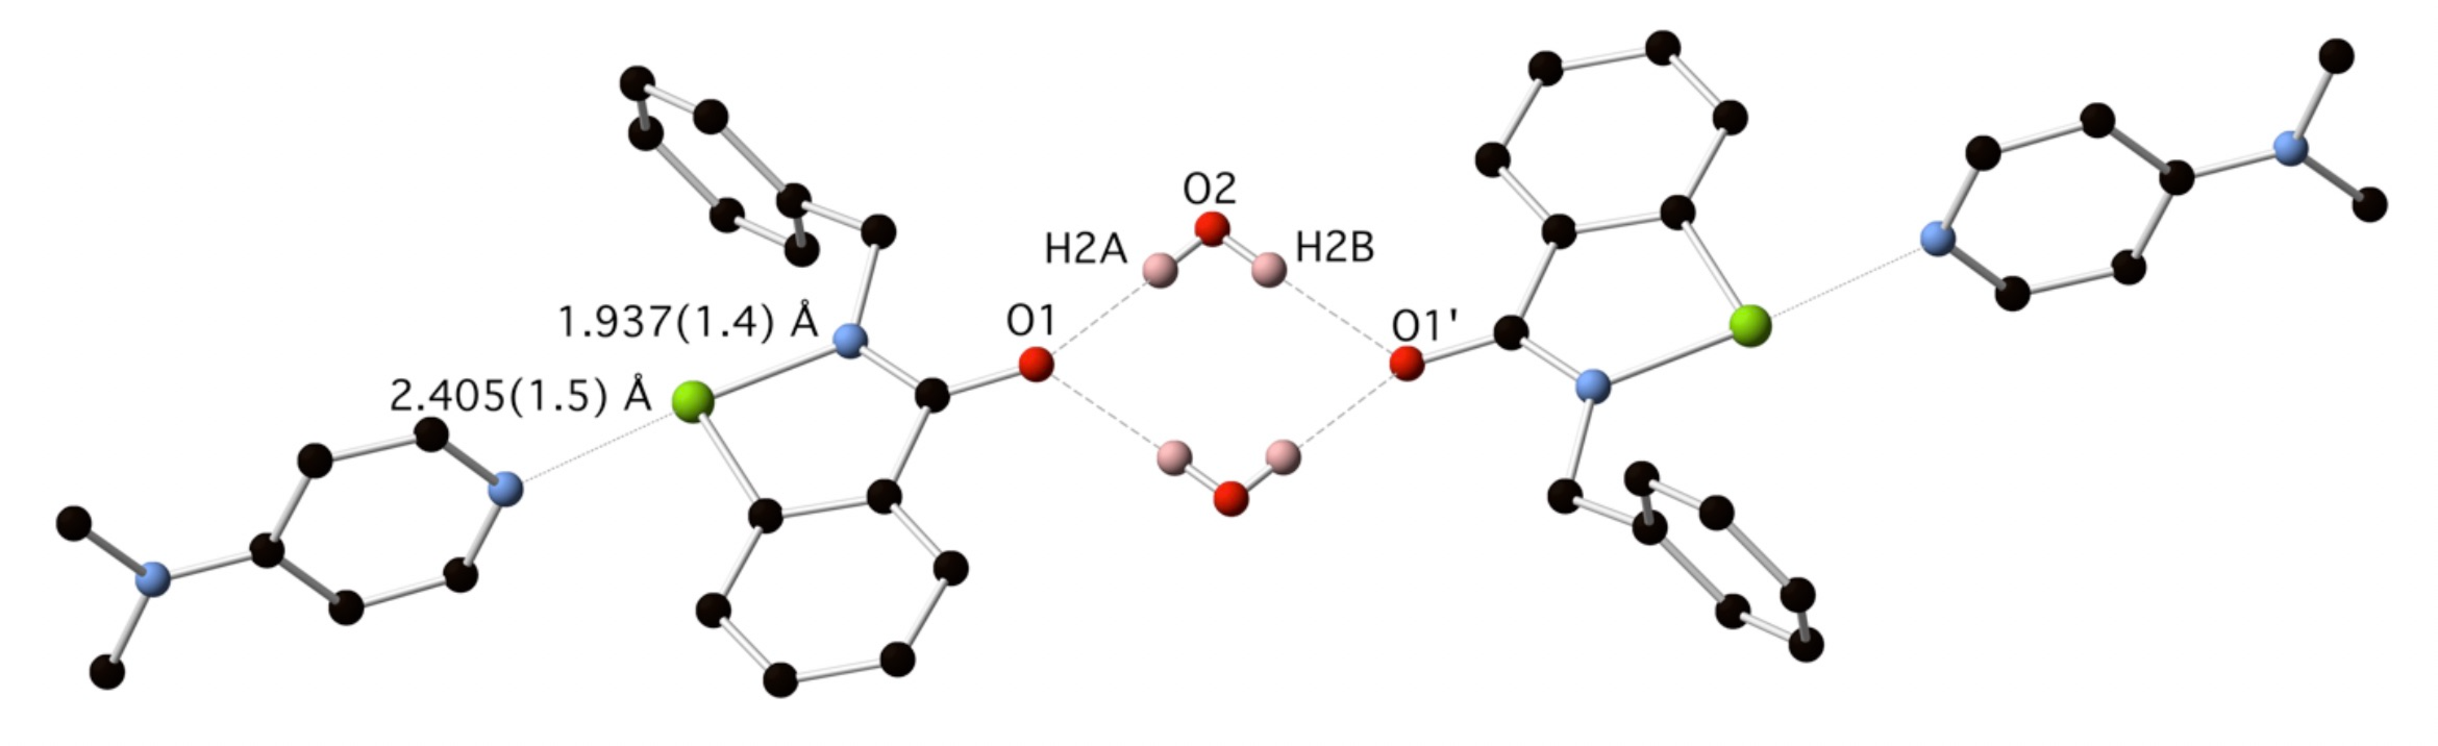
\includegraphics[width=0.8\linewidth]{Figures/benzyl-dmap-hydrate.pdf}
    \caption{Structure of \refcmpd{ebs.bn}$ \cdot $DMAP$ \cdot $\ce{H2O}.}
  \end{figure}

Subsequent investigations into derivatives where the electron demand of the Ch-bond donor was varied showed similar trends in both Ch-bond and endocyclic bond length (\cref{sec:hammett}).
This definitively demonstrated that the strength of the Ch-bond is (inferred from the bond length) determined by the degree of partial positive charge on the selenium atom.
To show the link between bond length and strength, we determined bond energies by NMR titration for a number of derivatives, which demonstrated the correlation and validated our used of bond length as a proxy for strength.
In this investigation we were able to obtain very high quality crystallographic data that allowed us to measure the valence electron density in the crystals.
This electron density was analysed within the QTAIM framework, which suggested that, in spite of the observed endocyclic bond lengthening, Ch-bonding was actually predominantly closed-shell in origin.
This conclusion was reached on the basis of the value of the Laplacian of the electron density at the bond critical point $\nabla^2 \rho_{\text{BCP}}$, which was positive, indicating that electron density was depleted between the Se and N atoms.

\begin{figure}
\centering
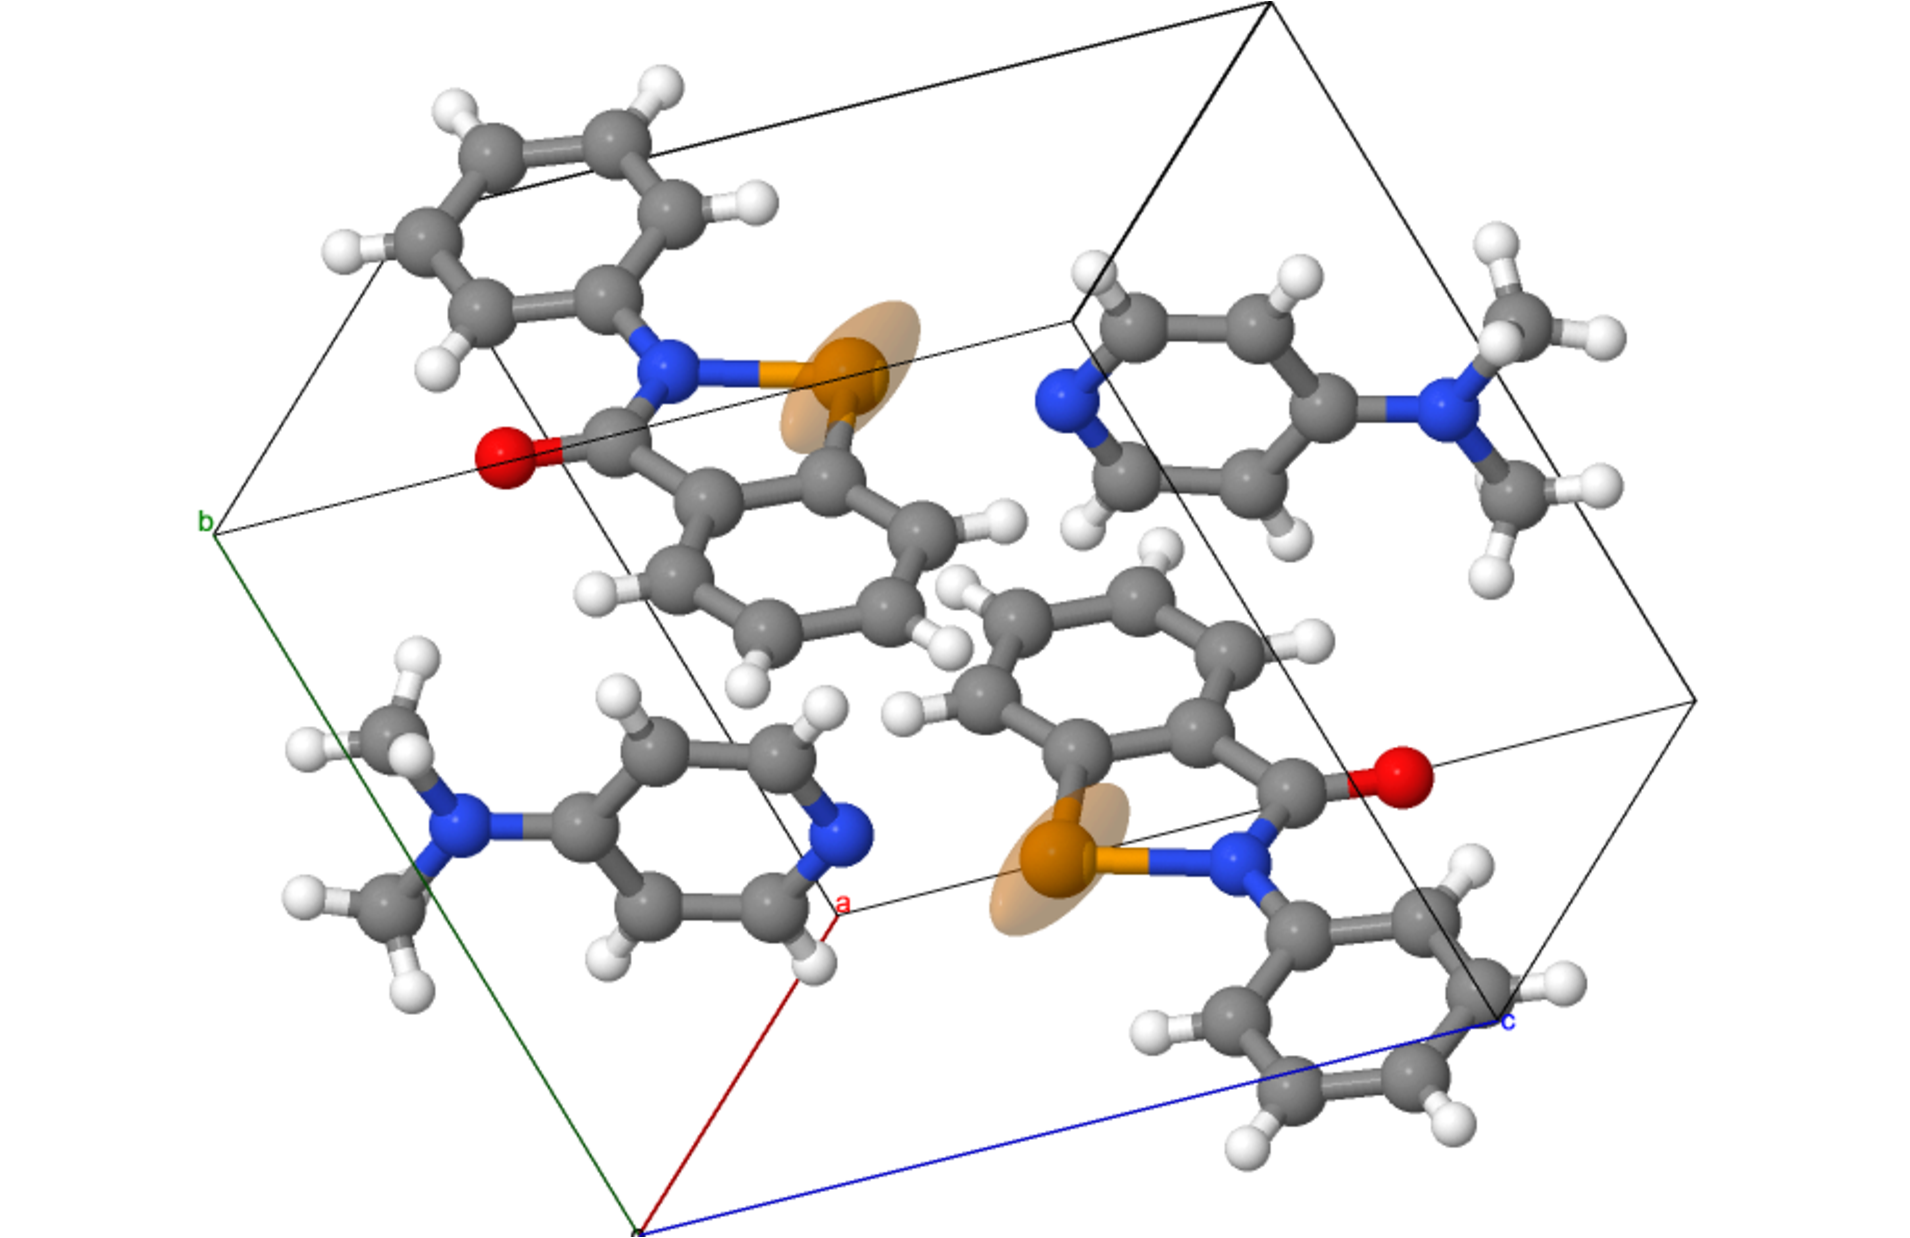
\includegraphics[width=0.7\linewidth]{Figures/expt-tensor-ebs-dmap.pdf}
\caption{Experimentally determined chemical shift tensor for \refcmpd{ebs}$ \cdot $DMAP.}
\end{figure}

Although single crystal x-ray diffraction is a powerful tool for the characterisation of Ch-bonded systems, it is not universally applicable as it requires a relatively large single crystal.
This may be unfeasible for systems such as polymers or biomolecules, so we sought alternative methods to characterise our complexes, in the hope that they might be useful for less trivial systems.
Solid state NMR represented one possible solution, as the chemical shift of selenium is extremely sensitive to changes in the electronic environment due to Ch-bonding.
Using this technique, we measured the chemical shift tensor of a series of complexes spanning the range of electron demand, all of which showed massive anisotropy.
Measurement of the orientation of the tensor in a single crystal showed that the selenium atom was strongly shielded in the direction of the Ch-bond, due to the approach of the lone pair, while it was deshielded orthogonal to this by the ring current of the aromatic systems.
GIAO calculations demonstrated that the tensor undergoes a substantial change in response to the approach of a Lewis base, which can be measured in a powder (non-oriented) spectrum, thus demonstrating that NMR can indeed be used to study Ch-bonding.
We also attempted to isolate a Ch-bonded complex in the gas phase, which we were able to do using a negatively charged Lewis base.
Low energy CID of this complex recovered the ion of the Lewis base, providing strong structural evidence that the complex was bound by a Ch-bond.

\begin{figure}
	\centering
	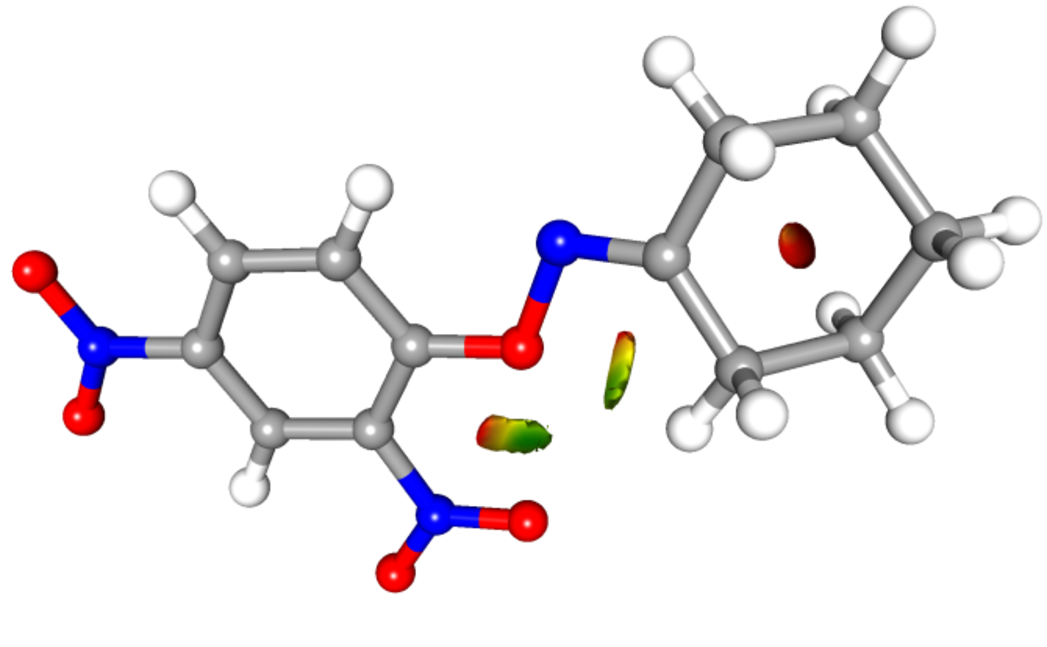
\includegraphics[angle=90,width=0.35\columnwidth]{Figures/cyclohexanone-oxime-dnp-nci.pdf}
	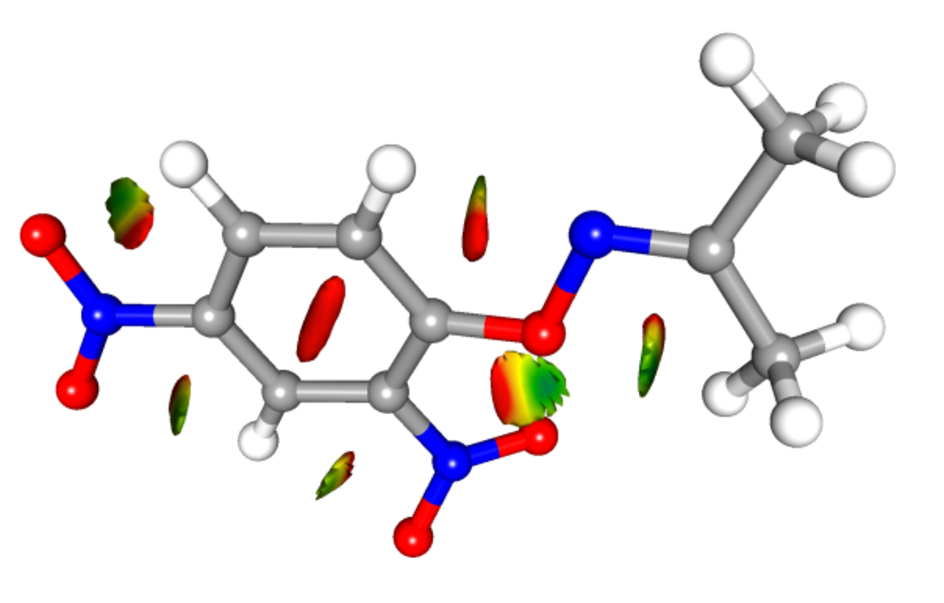
\includegraphics[angle=90,width=0.35\columnwidth]{Figures/acetone-oxime-dnp-nci.pdf}
	\caption[NCI maps for \refcmpd{cyclohexanone-oxime-dnp} and \refcmpd{acetone-oxime-dnp}.]{NCI maps for \refcmpd{cyclohexanone-oxime-dnp} and \refcmpd{acetone-oxime-dnp}. Positive values (non-bonding) are shown in red, and negative values (attractive) are shown in blue.}
\end{figure}

Most work on Ch-bonding to date has been focussed on sulfur, selenium, adn tellurium based donors.
These atoms are easily polarisable (therefore generate positive $\sigma$-holes), and selenium appears to be the ``sweet spot'' in terms of strength of Ch-bond versus ease of synthesis and toxicity.
Oxygen has recently been shown to act as a Ch-bond donor in highly activated systems such as \ce{OF2}, however we reported in \cref{sec:o-ch-bonding} a \textit{o}-nitro-O-aryl oxime which displays an \ce{O \cdots O} contact with features consistent with a Ch-bond.
We characterised this oxime, and a variety of derivatives, using high-resolution single crystal x-ray diffraction, and the resulting electron density supported our hypothesis that the contact was indeed due to Ch-bonding.
Further evidence was obtained in the form of a statistically significant lengthening of the \ce{O-N} oxime bond (corresponding to a n(O)$ \rightarrow \sigma^{\star} $(\ce{O-N}) delocalisation), which was supported by NBO calculations.
We attempted to manipulate both the Ch-bond donor and acceptor strengths in \cref{sec:o-ch-bonding-further}, to evaluate whether the expected structural effects would manifest.
Indeed, reducing the Ch-bond donor ability of the oxime (by making it more electron rich) ``switched off'' the Ch-bond, which was evident in the torsion of the nitro group.
The attraction due to Ch-bonding was overcome by exchange repulsion between the oxygens.
We also showed that the Ch-bond could be ``switched on'' again, by increasing the electron density at the nitro group, thus turning it into a better acceptor.
We believe these results are sufficient to claim Ch-bonding can indeed occur at oxygen.

\begin{figure}
    \centering
    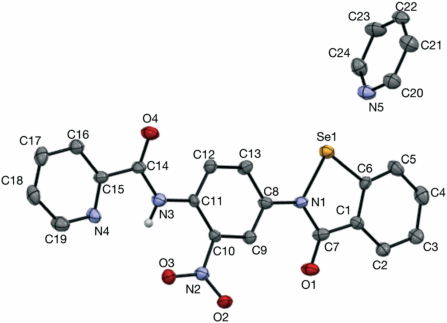
\includegraphics[width=0.8\linewidth]{Figures/ebs-nitroamide-2py-py-xtal.pdf}
    \caption{Thermal ellipsoid plot of \refcmpd{ebs-nitroamide-2py}$\cdot$pyridine.}
\end{figure}

We sought to exploit Ch-bonding to develop a DNA binding radioprotector, using the first-principles information we had obtained through our previous studies.
An analogue of the bis-benzimidazole Hoechst 33342 was envisaged, with one of the H-bond donor benzimidazoles replaced by a Ch-bonding benzisoselenazolinone, as in ebselen.
A late stage intermediate in an early synthetic route proved to exhibit interesting crystal packing, and this was investigated in \cref{sec:thermal-conversion}.
When recrystallised from pyridine, the solvent occupied one dimensional pores in the lattice, and was held in place via Ch-bonding.
TGA revealed that the pyridine was lost at a temperature of around 80\degree{}C, and variable temperature powder diffraction showed that the pyridine solvate converted smoothly to a de-solvate form, which could also be obtained by recrystallisation from DMF.
This transformation was accompanied by a rearrangement in Ch-bonds, in which the Ch-bonding requirement in the de-solvate was fulfilled by the carbonyl oxygen of an adjacent molecule.
We believe that this is interesting from a materials chemistry perspective, as it shows that Ch-bonding may be able to modulate the properties of void spaces in porous materials.

We were able to prepare the desired DNA binder via another method, and we attempted to characterise its interaction with DNA both crystallographically and spectroscopically (\cref{ch:dna-binder}).
Unfortunately, we were unable to obtain a co-crystal structure of the binder and a DNA oligomer, as it appeared to form an insoluble complex.
We also observed this precipitation in a UV-vis titration experiment.
Analysis of the precipitate suggested it contained nucleic acid material as well as the binder, and we attributed its formation to a covalent complex, which is understood to be a major pathway of action for ebselen derivatives.

While this hurdle could theoretically be overcome by tuning the electron density at the selenium, we were not able to investigate this further due to time constraints, compounded by the lack of access to lab facilities during the 2020 COVID-19 lockdown.
Instead, we turned to computational modelling of ebselen derivatives in biological systems.
While we have used DFT and ab initio methods to investigate Ch-bonding in previous chapters, these methods do not scale well, and are not widely used for the simulation of biomolecules and pharmaceutical development.
Molecular mechanics is almost universally used to model these systems, which relies on a force-field to describe bonding and non-bonding interactions.
As we have demonstrated numerous times, the chemistry of ebselen and its derivatives is dominated by Ch-bonding, however this is not modelled in standard force fields.
We therefore developed an extension to the Generalized Amber Force Field which simulates Ch-bonding by modelling the $\sigma$-hole as a positively charged pseudoatom on the surface of the selenium, and this work is detailed in \cref{sec:ebs-param}.
This gives realistic gas phase geometries, and also accurately reproduces the crystal packing and density of solid ebselen.
We also validated our model against a known ebselen target, and the crystallographic binding pose was accurately reproduced.

\section{Future work}


\printbibliography[heading=subbibliography]
\end{refsection}
